\section{Metodi e Modelli}

Nell'ambito di questa ricerca, l'approccio adottato è stato incentrato 
sulla prospettiva di modellare il problema specifico all'interno del 
contesto di una rete sociale. L'obiettivo principale di questa indagine 
è stato quello di analizzare e comprendere il processo di diffusione di 
una pandemia virale all'interno di un ambiente concreto, il quale è 
principalmente costituito da punti di interesse (PdI) interconnessi tra 
loro attraverso una struttura di collegamenti, rappresentata graficamente 
sotto forma di un grafo. 

\begin{figure}[!hb]
	\centering
	\begin{subfigure}[b]{0.3\textwidth}
		\centering
		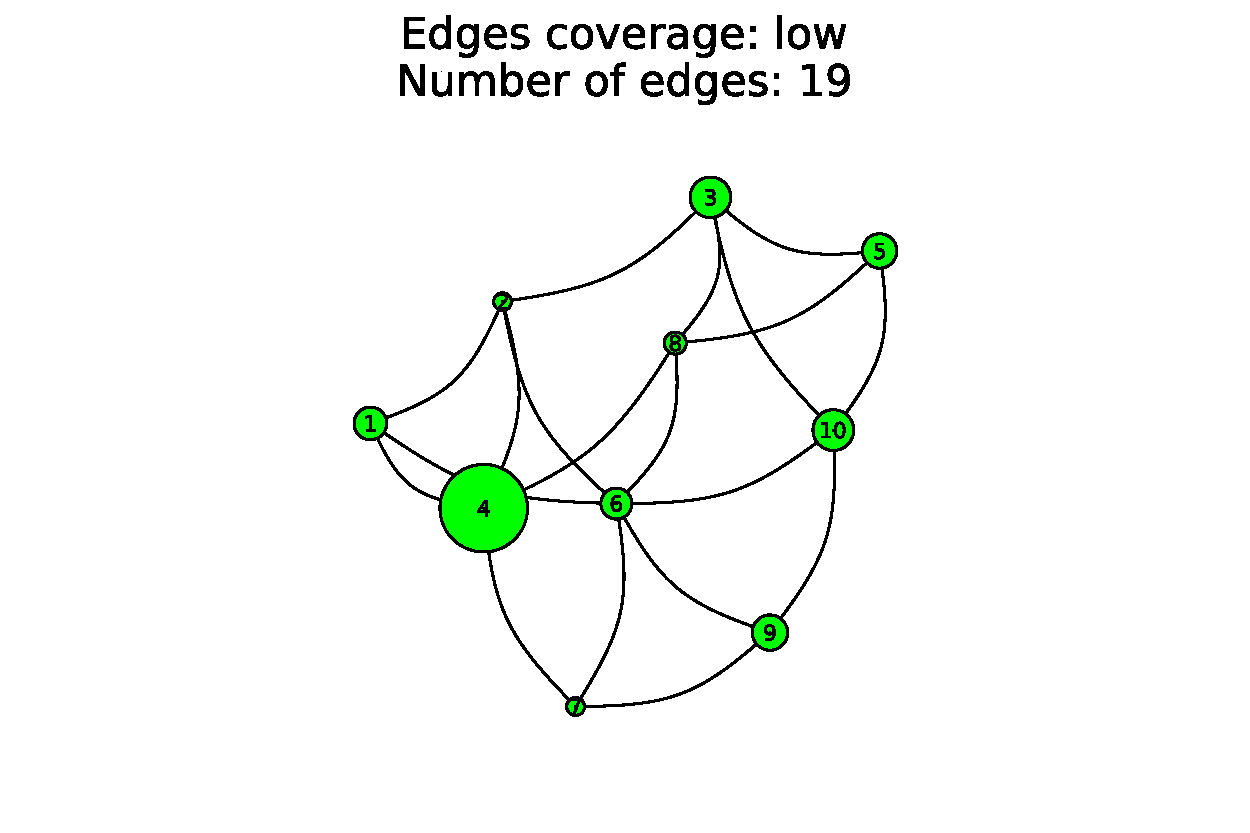
\includegraphics[width=\textwidth]{img/low.pdf}
		\caption{Esempio di grafo connesso con copertura bassa}
		\label{fig:connected_graph_example_low}
	\end{subfigure}
	\hfill
	\begin{subfigure}[b]{0.3\textwidth}
		\centering
		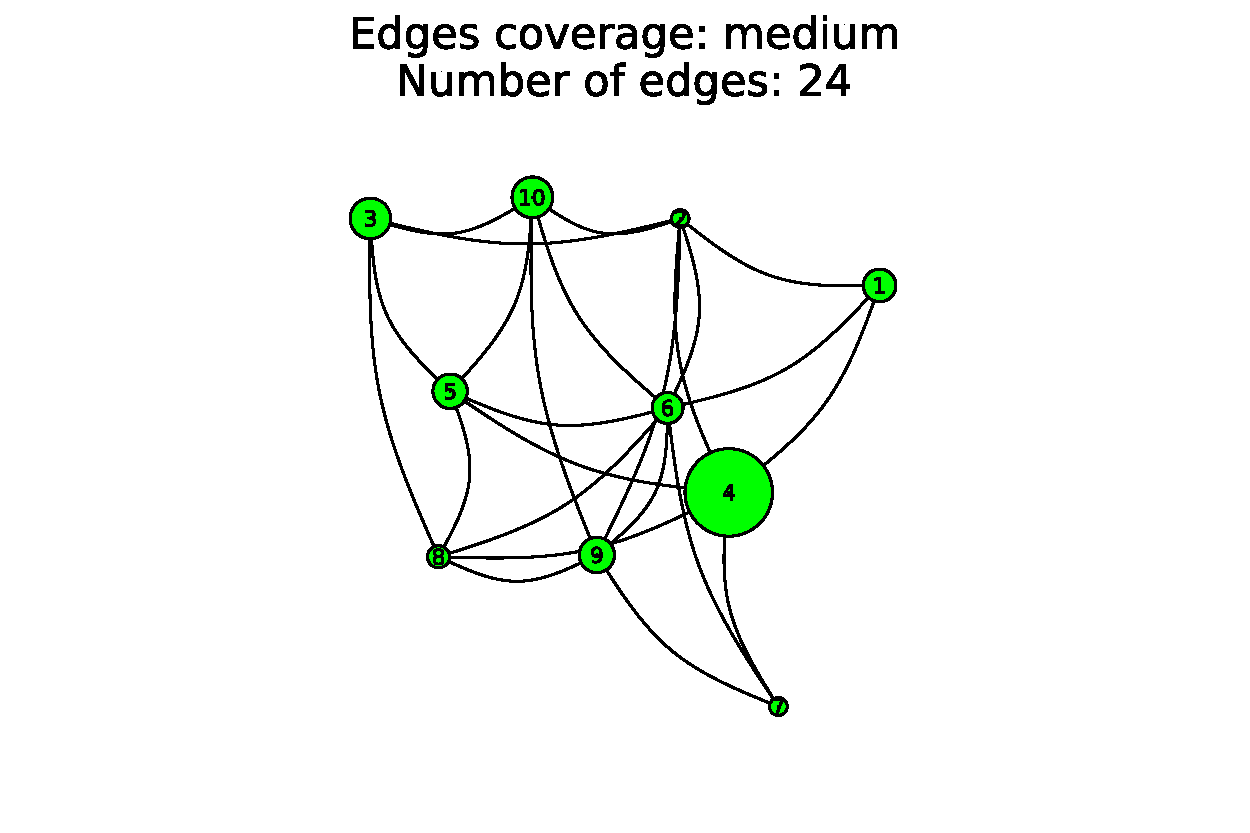
\includegraphics[width=\textwidth]{img/medium.pdf}
		\caption{Esempio di grafo connesso con copertura media}
		\label{fig:connected_graph_example_medium}
	\end{subfigure}
	\hfill
	\begin{subfigure}[b]{0.3\textwidth}
		\centering
		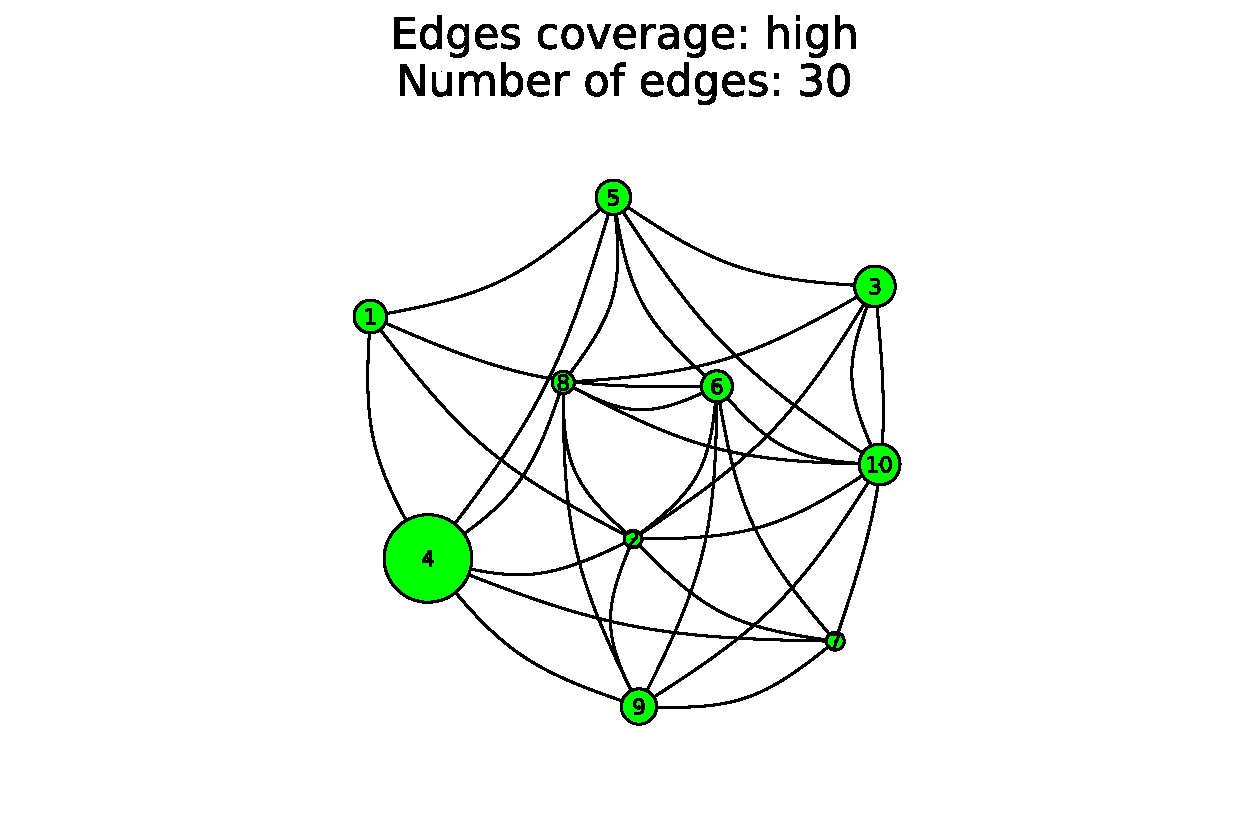
\includegraphics[width=\textwidth]{img/high.pdf}
		\caption{Esempio di grafo connesso con copertura alta}
		\label{fig:connected_graph_example_high}
	\end{subfigure}
\end{figure}

Questo approccio si avvicina a una prospettiva di tipo mesoscopico, 
orientata al macroscopico. La scelta di tale approccio deriva dalla 
necessità di modellare il sistema in maniera più ampia, concentrandosi 
sulla risposta collettiva di un agente astratto agli interventi mirati 
per contrastare l'epidemia in modo localizzato.

\subsection{Approccio con Rete Sociale}

Il modello sviluppato fa uso del framework "Agents.jl" \cite{Agents.jl} e 
definisce un modello ad agenti (ABM). In questo contesto, la struttura 
spaziale del modello non è rilevante, ma le connessioni tra gli agenti 
lo sono. Gli agenti vengono considerati come nodi all'interno di un grafo, 
in cui viene simulato il ciclo di vita della pandemia attraverso un 
modello SEIR deterministico. Gli agenti sono definiti come oggetti di tipo 
"ContinuousAgent", poiché lo spazio del modello è considerato continuo.

La struttura dell'agente è essenziale e include i seguenti campi principali:

\begin{itemize}
	\item \textbf{population}: un intero che rappresenta il numero totale 
	di individui presenti nel nodo.
	\item \textbf{status}: un vettore di numeri decimali che 
	rappresenta lo stato della popolazione nel nodo, espressa 
	come percentuale di individui.
	\item \textbf{param}: un vettore di numeri decimali che contiene 
	i parametri specifici del modello SEIR per il nodo.
	\item \textbf{happiness}: un campo di supporto per il bilanciamento 
	delle contromisure applicate dal controllore.
\end{itemize}

Questi campi costituiscono l'ossatura dell'agente e sono essenziali per 
la rappresentazione e la gestione delle dinamiche della pandemia 
all'interno del sistema modellato.

\subsubsection*{Grafo Sociale}

Un grafo sociale è una struttura dati utilizzata per rappresentare in 
maniera formale le complesse relazioni sociali che sussistono tra diverse 
entità all'interno di una comunità o di un sistema. In questo specifico 
contesto, i nodi del grafo fungono da rappresentazioni delle entità 
coinvolte, spesso individui, mentre gli archi tra questi nodi 
simboleggiano le relazioni sociali che legano tali individui tra loro.

Questa metodologia di rappresentazione è comunemente adottata per 
modellare le reti sociali, che costituiscono un settore di grande 
interesse in diverse discipline, come sociologia, informatica, e analisi 
delle reti. Nell'ambito delle reti sociali, gli individui stessi sono 
considerati i nodi del grafo, mentre le connessioni tra di essi vengono 
tradotte in archi. Questo approccio consente di analizzare e studiare 
una vasta gamma di fenomeni sociali, inclusi processi di diffusione 
dell'informazione, dinamiche di influenza reciproca, 
formazione di comunità, e molte altre interazioni sociali complesse.

\begin{minipage}{\linewidth}
    \centering
    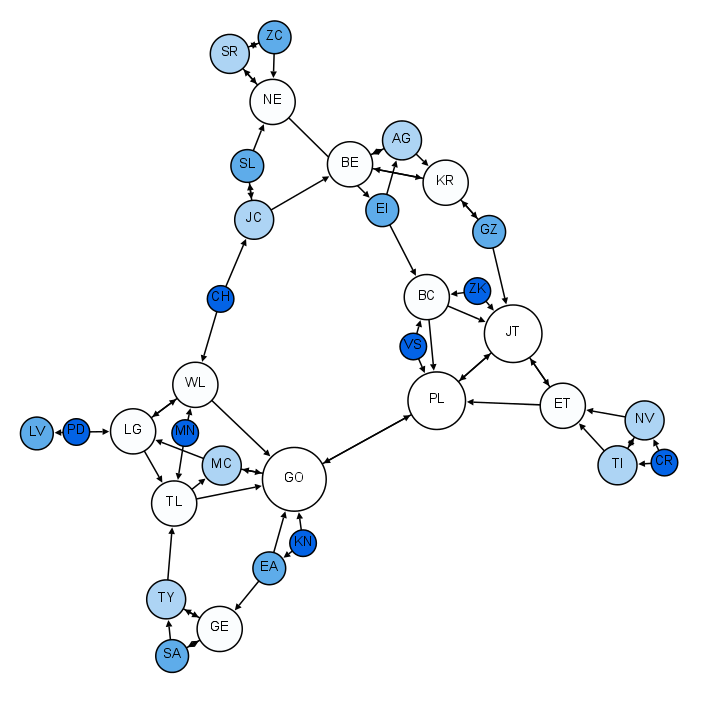
\includegraphics[width=\textwidth]{img/Moreno_Sociogram_3rd_Grade.png}
    \captionof{figure}{Moreno's Sociagram of a 3rd grade class}
	\url{https://en.wikipedia.org/wiki/Sociogram#/media/File:Moreno_Sociogram_3rd_Grade.png}
    \label{fig:social_graph}
\end{minipage}
\newpage

\subsection{Agente}

Per una comprensione più approfondita dei concetti esposti, 
si può esaminare ulteriormente l'implementazione dell'agente in questione. 
Quest'ultimo è stato concepito con una struttura minimale, 
ridotta ai soli attributi strettamente essenziali per il suo corretto 
funzionamento. Tali attributi costituiscono l'ossatura di base che 
consente all'agente di interagire con l'ambiente circostante e con 
altri agenti all'interno del sistema.

Nel contesto dell'evoluzione degli agenti, è fondamentale notare che 
questa si svolge in maniera indipendente rispetto agli altri agenti 
presenti nel medesimo contesto. Tale indipendenza è regolamentata da un 
sistema di equazioni differenziali ordinarie (ODE), che rappresenta il 
cuore del processo decisionale dell'agente. 
Tuttavia, è cruciale sottolineare che, nonostante questa indipendenza, 
l'agente non opera in un isolamento completo.

Le interazioni tra agenti sono agevolate dalle connessioni esistenti 
tra i nodi del grafo, che possono essere interpretate come canali di 
comunicazione o canali attraverso i quali fluiscono influenze e 
informazioni. Inoltre, la matrice di migrazione rappresenta un elemento 
importante in questo contesto. Essa definisce come l'agente può essere 
influenzato da altri agenti all'interno della stessa rete. 
Questo meccanismo consente un grado di adattamento e cooperazione tra 
agenti, sebbene ognuno di essi mantenga la propria autonomia decisionale
(Figura \ref{fig:migration_matrix_function}).

\begin{minipage}{\linewidth}
    \centering
    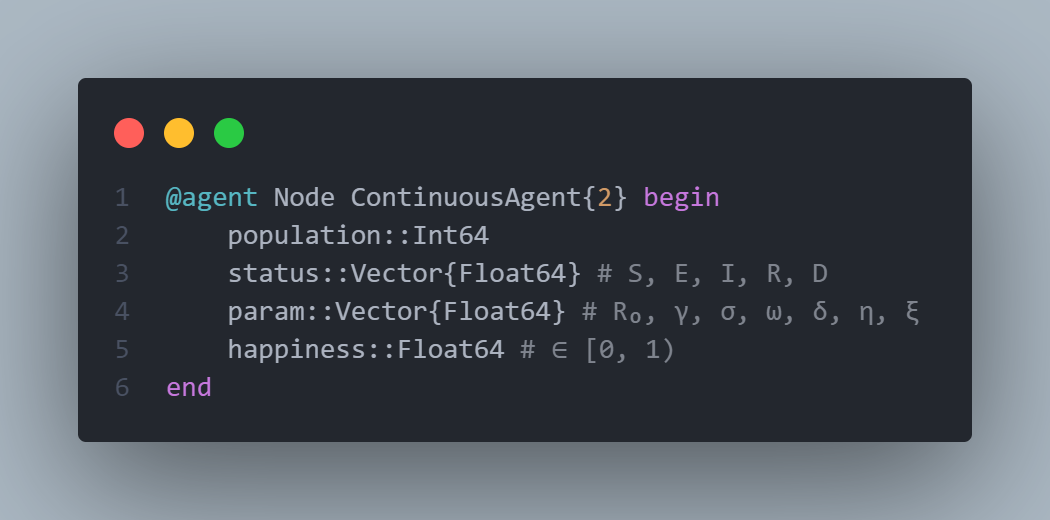
\includegraphics[width=\textwidth]{img/node_agent.png}
    \captionof{figure}{Codice Agente}
    \label{fig:Agent_code}
\end{minipage}
\newpage

\subsection{Spazio e Modello}
Lo spazio del modello è fondato su un grafo connesso, il cui numero 
di archi è determinato in base alla copertura desiderata degli archi. 
La topologia specifica del grafo viene creata in conformità alle 
preferenze dell'utente, rispettando un limite inferiore imposto dalla 
connessione minima e un limite superiore rappresentato dalla connessione 
completa.

In altre parole, il grafo che costituisce il contesto spaziale del 
modello è progettato in modo dinamico per adattarsi alle esigenze e 
alle scelte dell'utente. Queste preferenze determinano sia il grado di 
interconnessione tra gli agenti (nodi del grafo) sia la forma generale 
del grafo stesso. Il limite inferiore garantisce una connessione minima 
tra gli agenti, mentre il limite superiore consentirebbe la massima 
interconnessione possibile, ovvero una situazione in cui ogni agente è 
connesso a tutti gli altri.

\begin{figure}[!hb]
	\centering
	\begin{subfigure}[b]{0.45\textwidth}
		\centering
		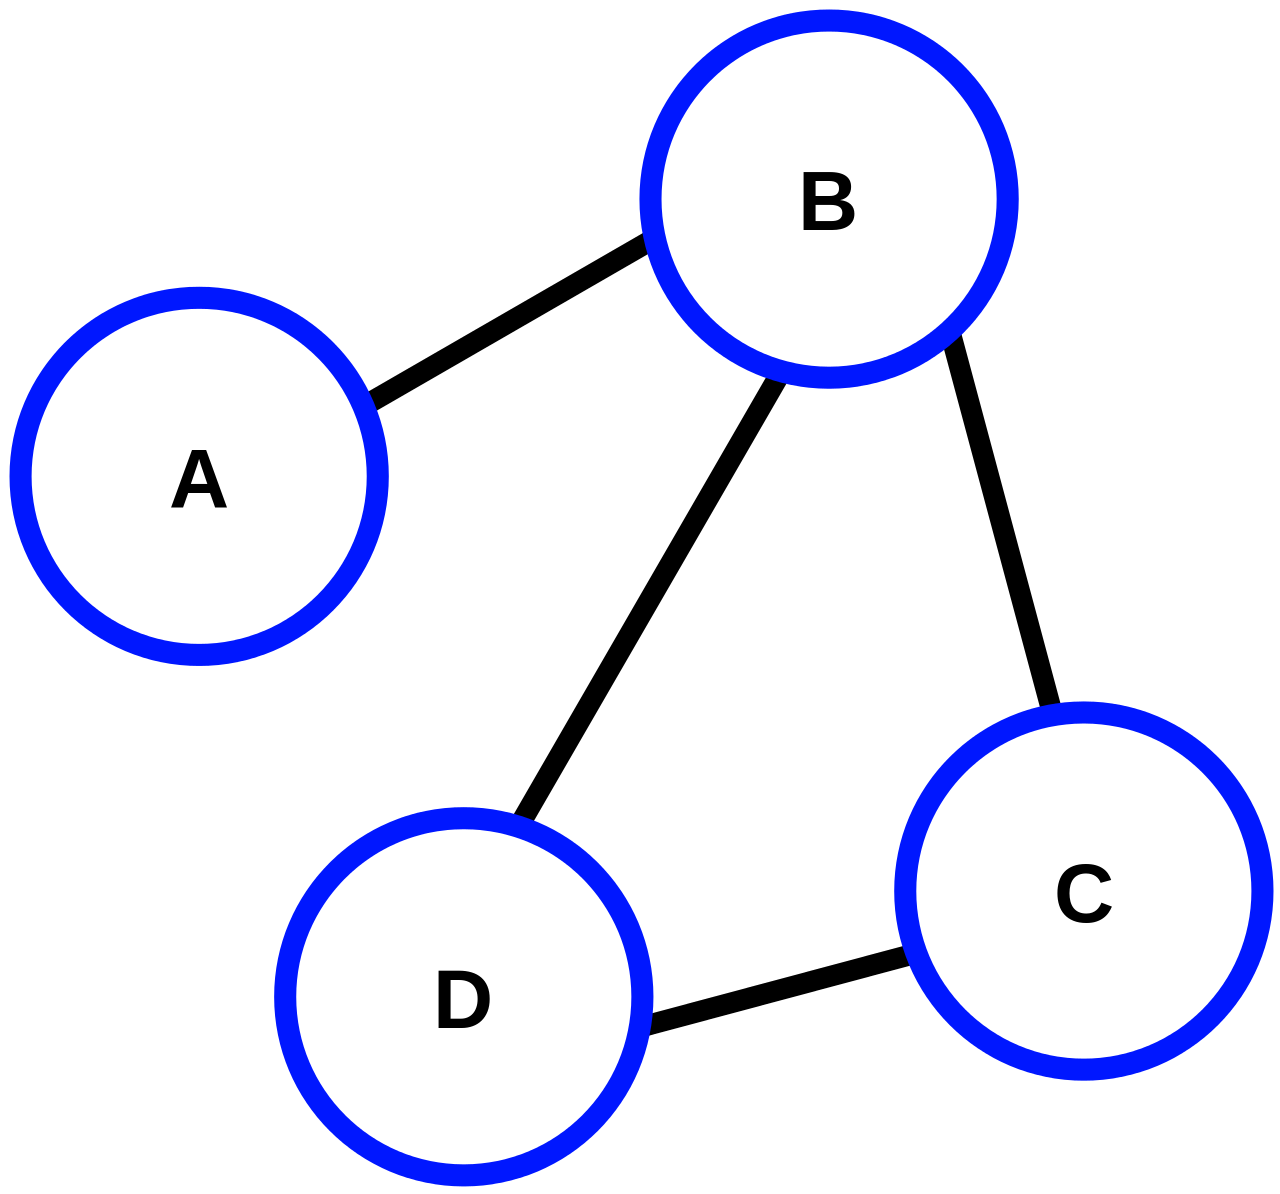
\includegraphics[width=\textwidth]{img/CPT-Graphs-undirected-unweighted-ex1.svg.png}
		\caption{Esempio di grafo connesso}
		\url{https://it.wikipedia.org/wiki/Grafo_connesso#/media/File:CPT-Graphs-undirected-unweighted-ex1.svg}
		\label{fig:connected_graph_example}
	\end{subfigure}
	\hfill
	\begin{subfigure}[b]{0.45\textwidth}
		\centering
		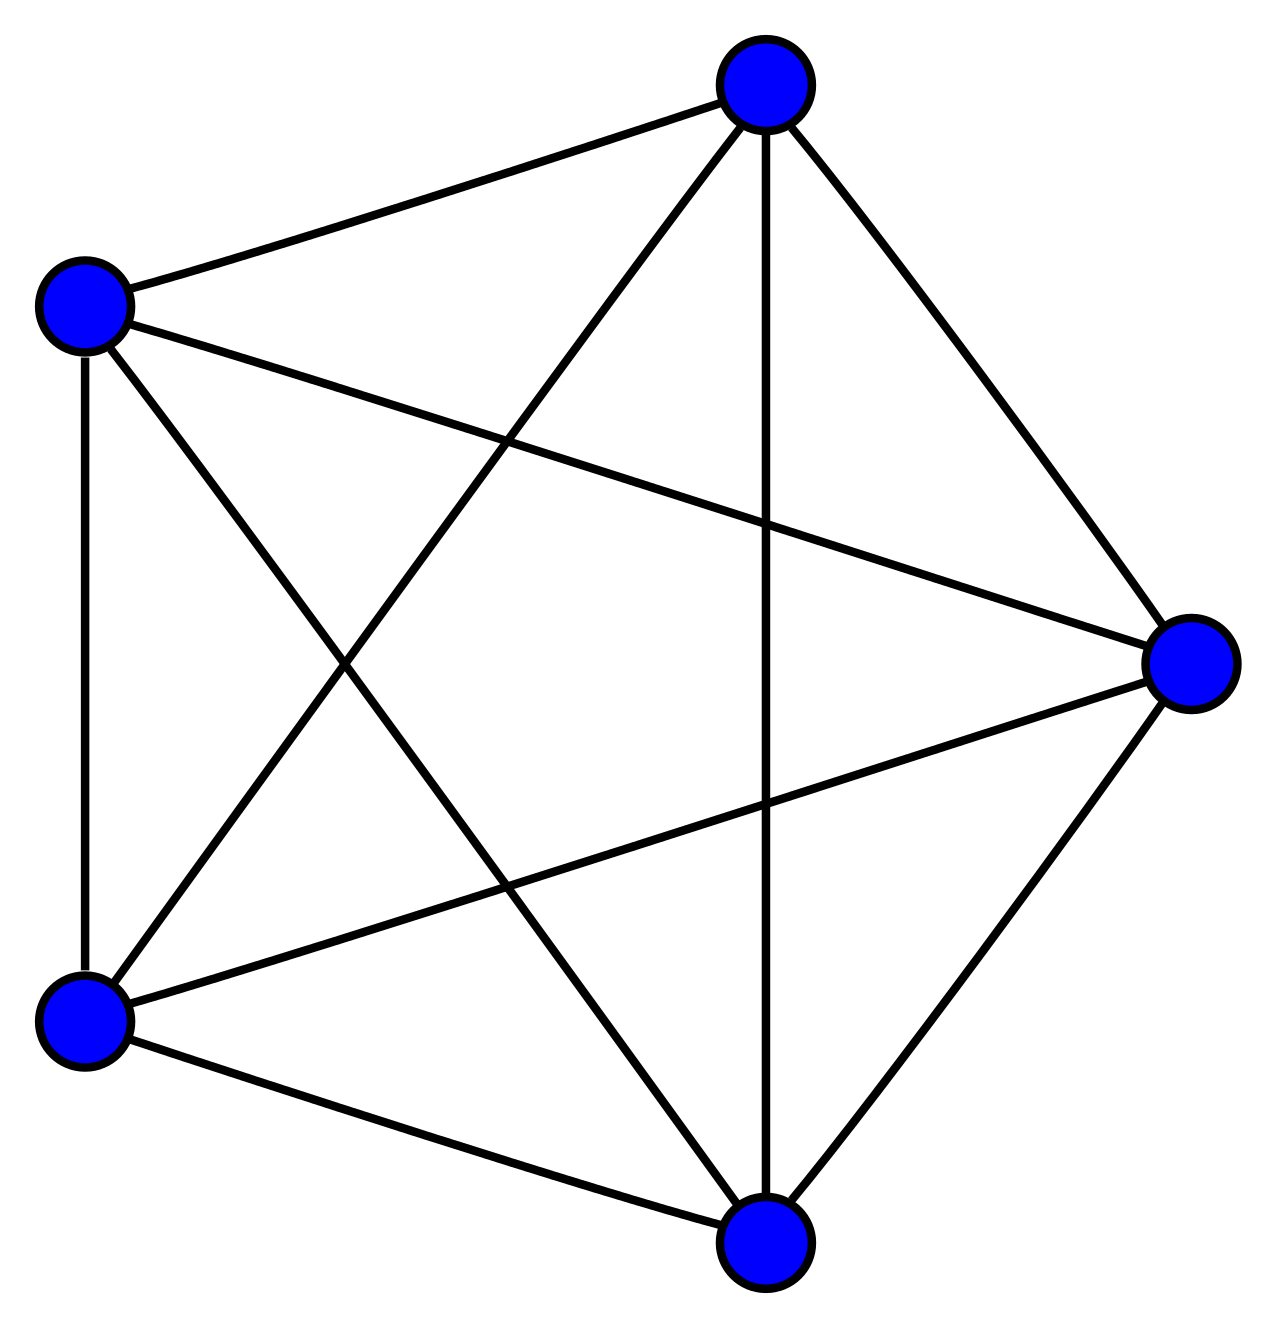
\includegraphics[width=\textwidth]{img/4-simplex_graph.svg.png}
		\caption{Esempio di grafo completo}
		\url{https://en.wikipedia.org/wiki/Complete_graph#/media/File:4-simplex_graph.svg}
		\label{fig:complete_graph_example}
	\end{subfigure}
\end{figure}

Questo approccio flessibile alla creazione della topologia del grafo 
permette agli utenti di configurare il modello in modo adatto alle 
specifiche condizioni e alle variabili in gioco, fornendo così un 
livello di personalizzazione che può essere fondamentale per la 
comprensione e la modellazione dei fenomeni legati alla diffusione della 
pandemia virale all'interno del sistema.

\begin{minipage}{\linewidth}
    \centering
    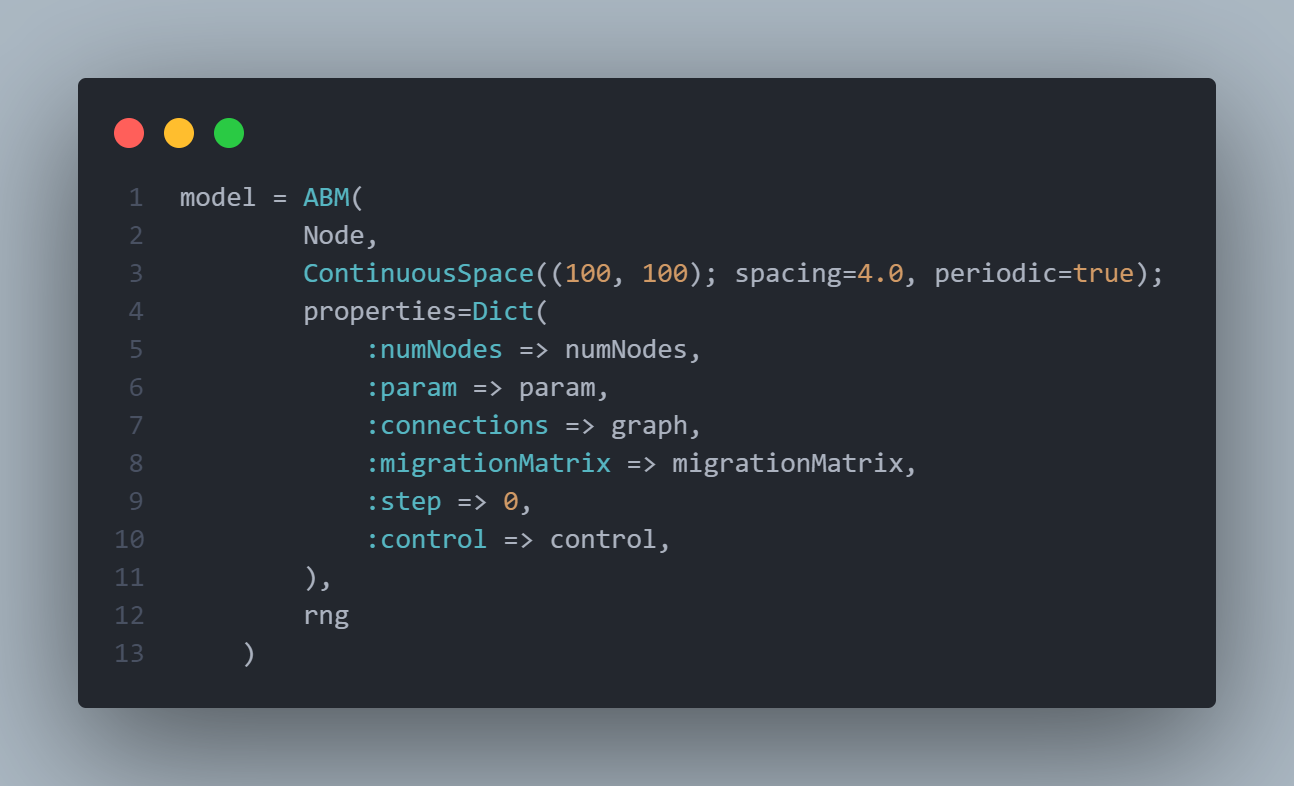
\includegraphics[width=\textwidth]{img/sngraph_model.png}
    \captionof{figure}{Codice Modello}
    \label{fig:Model_code}
\end{minipage}

\subsection{Funzione di Avanzamento Agente}

Ogni agente all'interno del modello adotta un ciclo di comportamento che 
incorpora tre compiti fondamentali:

\begin{itemize}
	\item \textbf{Spostamento tra i nodi del grafo} \cite{Ding2021}: 
	Gli agenti seguono un sistema di spostamento all'interno della rete, 
	il quale può essere influenzato da fattori variabili, 
	come ad esempio la topologia del grafo, la preferenza dell'agente, 
	o dinamiche specifiche del modello. Questo aspetto del 
	comportamento dell'agente è influenzato da un processo di 
	spostamento tra i nodi del grafo, e tali movimenti possono essere 
	utilizzati per modellare gli spostamenti fisici degli individui in 
	un contesto di pandemia.
	\item \textbf{Calcolo del proprio "livello di felicità"}: Gli agenti 
	effettuano un calcolo che valuta il loro "livello di felicità". 
	Questo parametro può essere influenzato da molteplici fattori, 
	inclusi i dati relativi allo stato di salute, le misure di 
	intervento adottate, le connessioni sociali e le condizioni 
	ambientali. Il livello di felicità costituisce un indicatore 
	importante per comprendere la percezione e il benessere degli 
	agenti nell'ambiente simulato.
	\item \textbf{Chiamata al controllore per valutare le misure 
	di intervento necessarie}: Gli agenti comunicano con il controllore 
	al fine di valutare le misure di intervento necessarie. 
	Questo processo di valutazione considera l'evoluzione della pandemia, 
	il comportamento degli agenti e i parametri specifici del modello SEIR, 
	tra altri fattori. Le misure di intervento possono comprendere 
	restrizioni, vaccinazioni, consigli alla popolazione o altre 
	strategie atte a mitigare la diffusione del virus.
\end{itemize}

Questi tre compiti costituiscono una sequenza chiave di attività che 
ogni agente esegue ciclicamente all'interno del modello, contribuendo 
in modo significativo all'analisi della diffusione della pandemia e 
alla valutazione delle misure di intervento.

\begin{minipage}{\linewidth}
	\centering
	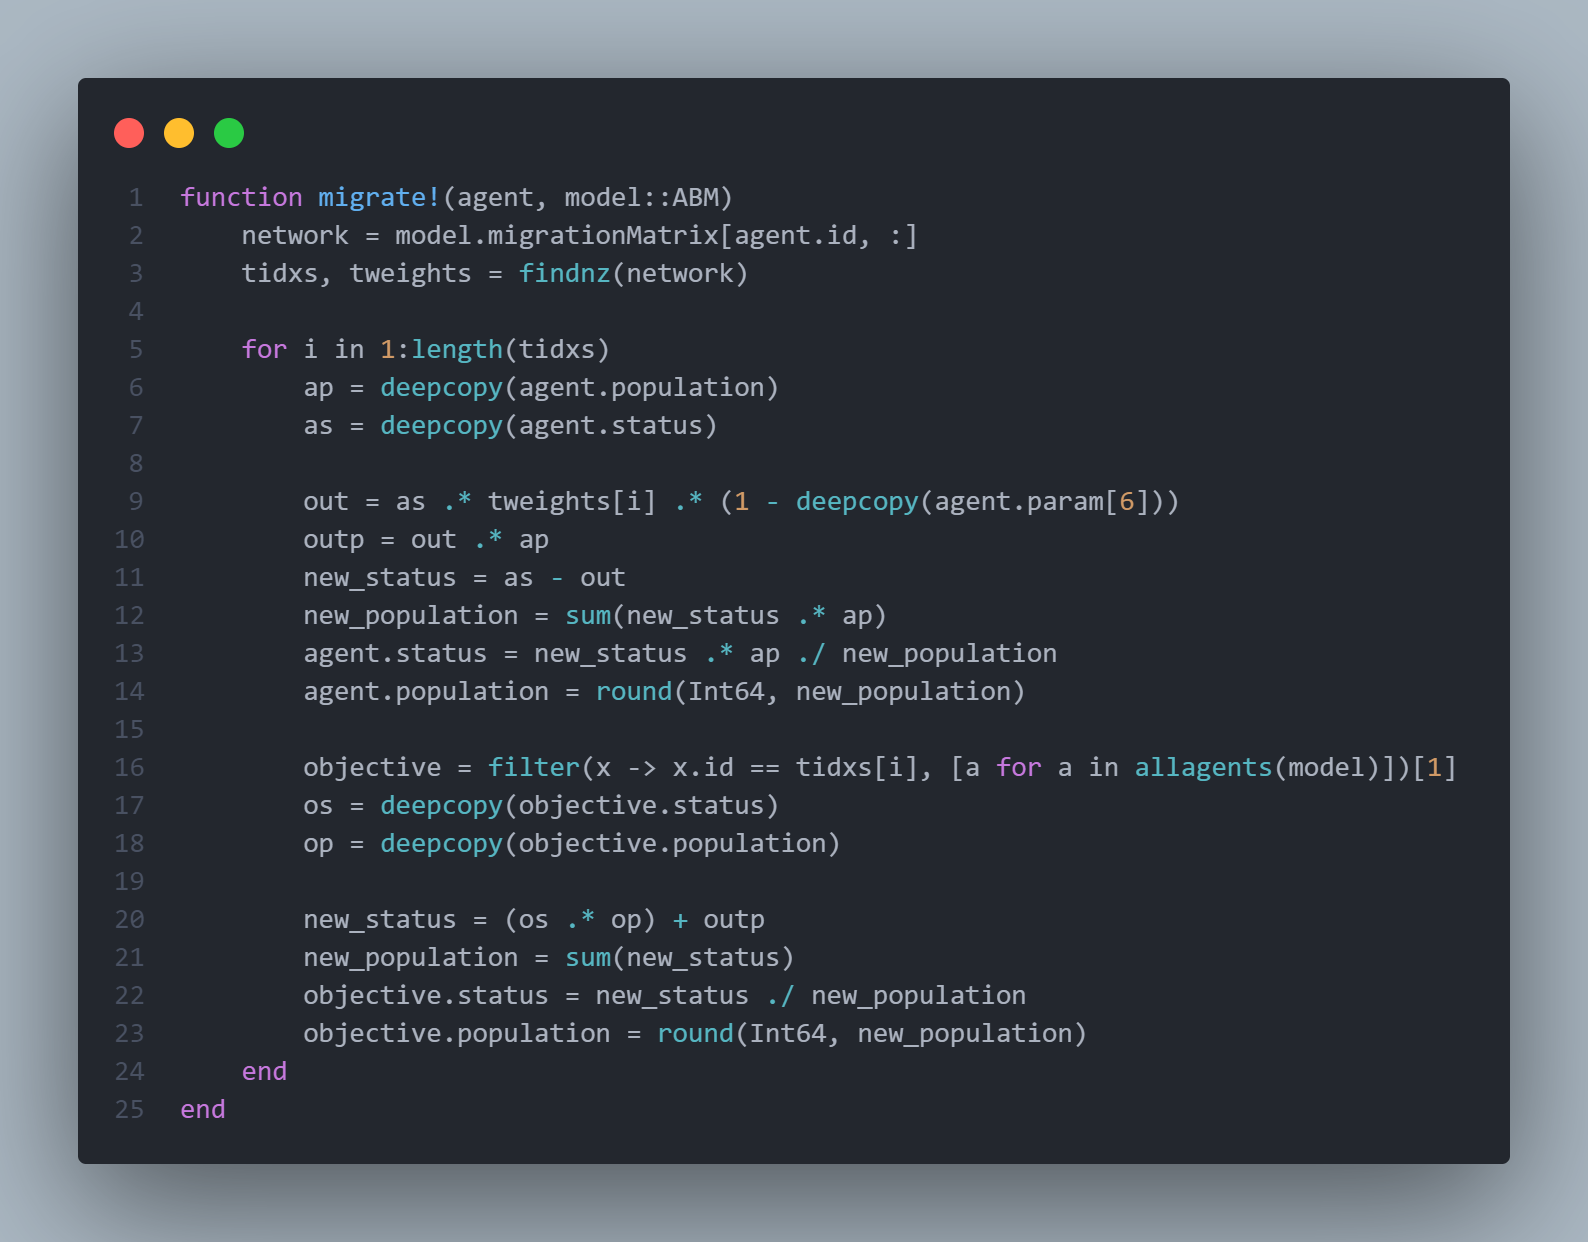
\includegraphics[width=\textwidth]{img/migratef.png}
	\captionof{figure}{Funzione atta a calcolare lo spostamento di agenti da un nodo all'altro del grafo}
	\label{fig:migrationf}
\end{minipage}

\begin{minipage}{\linewidth}
	\centering
	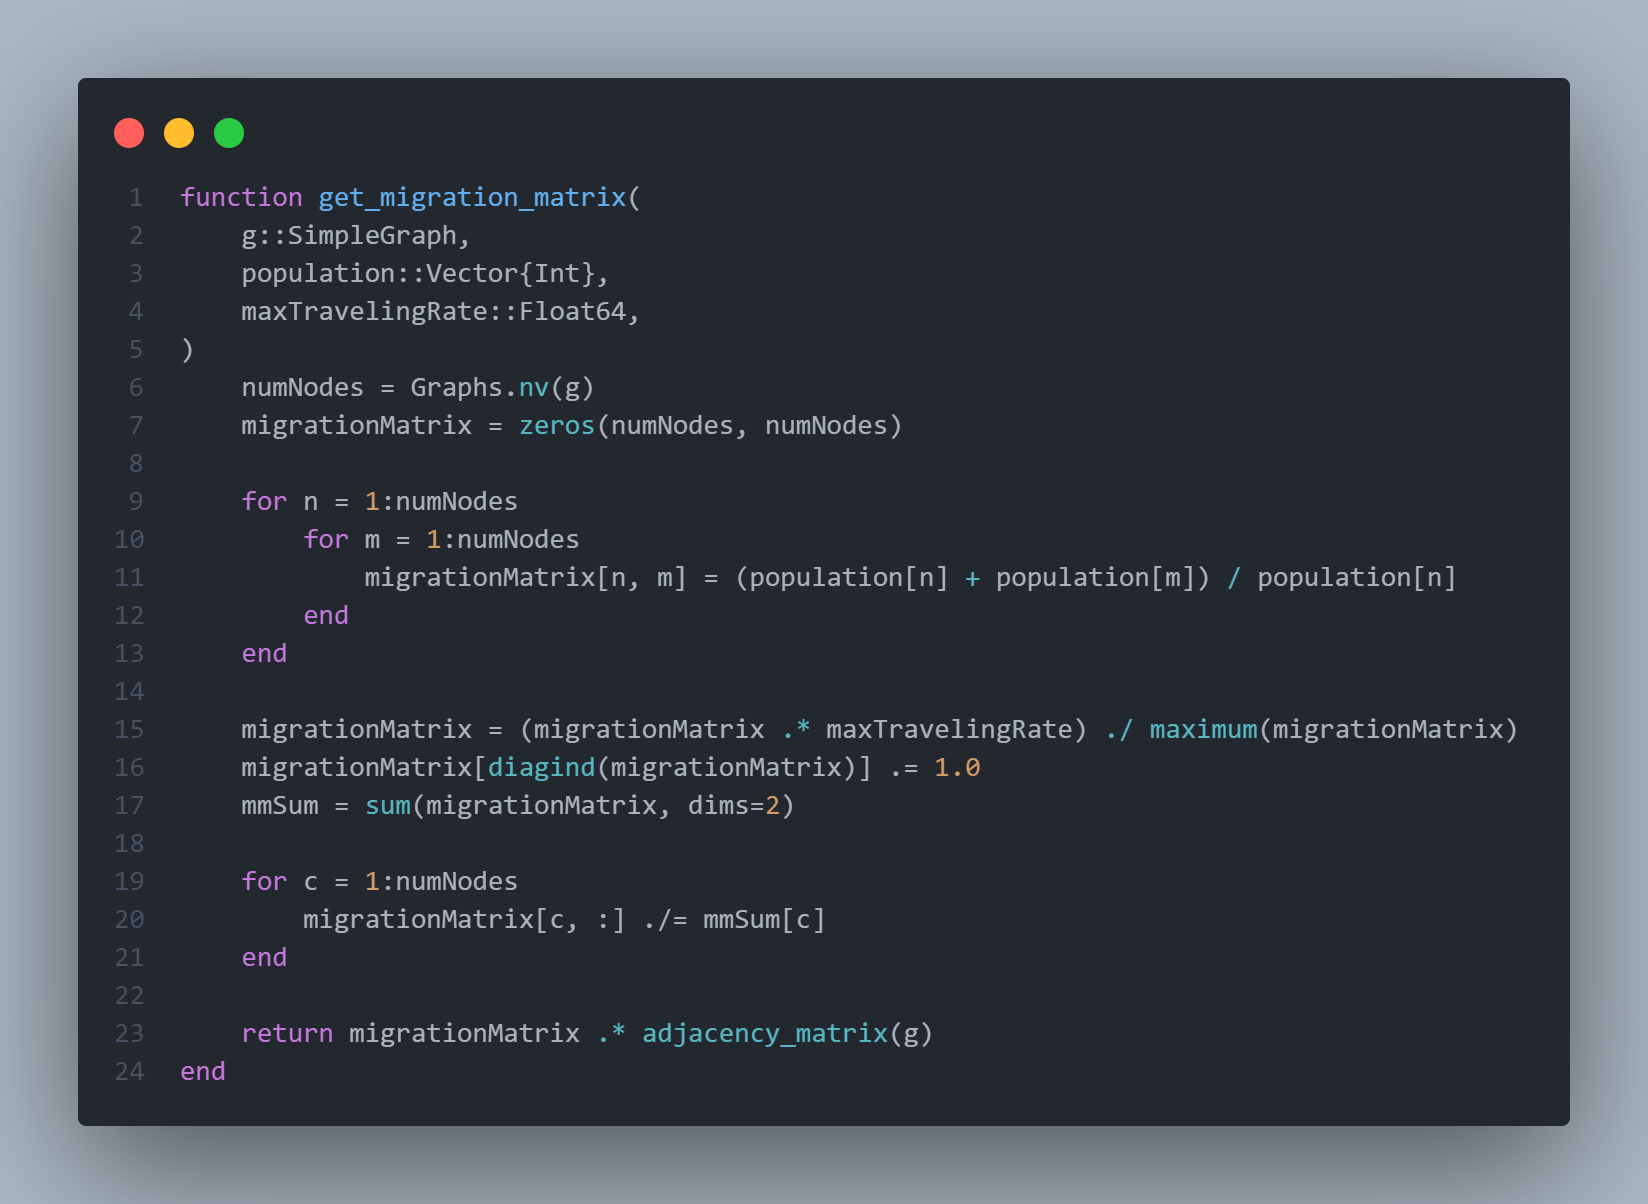
\includegraphics[width=\textwidth]{img/mmfunc.png}
	\captionof{figure}{Funzione che crea la matrice di migrazione data la topologia di un grafo}
	\label{fig:migration_matrix_function}
\end{minipage}

\begin{minipage}{\linewidth}
	\centering
	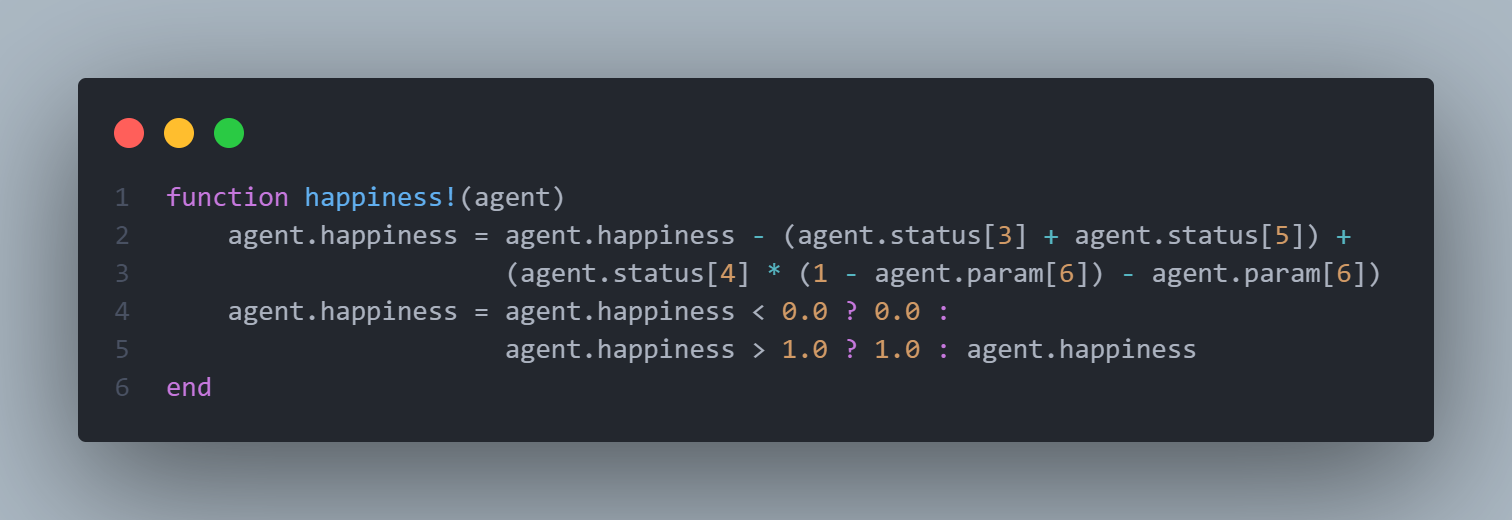
\includegraphics[width=\textwidth]{img/happiness.png}
	\captionof{figure}{Funzione atta a calcolare la felicità degli agenti}
	\label{fig:happinessf}
\end{minipage}
\newpage

\subsection{Funzione di Avanzamento Modello}

Il modello svolge un ruolo di coordinamento nell'evoluzione degli agenti 
e si occupa di operazioni che coinvolgono l'intero sistema, 
anziché focalizzarsi sugli agenti individuali. 
Queste operazioni includono principalmente due aspetti chiave:

\begin{itemize}
	\item \textbf{Aggiornamento delle equazioni differenziali 
	ordinarie (ODE)}: Il modello si fa carico dell'aggiornamento 
	delle equazioni differenziali ordinarie associate a ciascun agente. 
	Le ODE rappresentano il modello SEIR deterministico che guida 
	l'evoluzione della pandemia all'interno di ciascun agente. 
	L'aggiornamento di queste equazioni è cruciale per monitorare e 
	prevedere il comportamento del virus e dei suoi effetti sulla 
	popolazione.
	\item \textbf{Gestione delle varianti del virus di interesse}: Il 
	modello si occupa anche della gestione delle varianti del virus 
	di interesse. Questo include il monitoraggio delle mutazioni e 
	delle caratteristiche delle varianti, nonché l'aggiornamento dei 
	parametri del modello in base all'emergere di nuove varianti. 
	La gestione efficace delle varianti è essenziale per valutare in 
	modo realistico l'andamento della pandemia e determinare 
	l'efficacia delle misure di intervento.
\end{itemize}

\subsubsection{Funzione per la Generazione delle Varianti del Virus (VOC)}

La generazione delle Varianti di Interesse 
(VOC, acronimo di Variant of Concern) nel contesto del modello si 
basa su alcune assunzioni chiave. Tra queste assunzioni figurano:

\begin{itemize}
	\item \textbf{Tasso di mutazione casuale delle basi del virus}: 
	Si assume che le VOC si sviluppino principalmente a causa di 
	mutazioni casuali nelle basi del virus. Queste mutazioni possono 
	verificarsi durante la replicazione del virus, portando a nuove 
	varianti con caratteristiche genetiche leggermente diverse. 
	Tuttavia, questa rappresentazione semplificata del processo di 
	mutazione è un'approssimazione del comportamento reale delle 
	varianti, che coinvolge una gamma più ampia di fattori e processi 
	genetici.
	\item \textbf{Distribuzione dei parametri pandemici}: La generazione 
	delle VOC considera una distribuzione dei parametri pandemici, 
	il che significa che le varianti possono differire in termini di 
	infettività, gravità dei sintomi, periodo di incubazione, e così via. 
	Questa variabilità nei parametri pandemici riflette la diversità 
	delle varianti del virus nel mondo reale.
\end{itemize}

È importante notare che questa implementazione è volutamente 
semplificata per scopi di modellazione e simulazione. 
La realtà dei processi di mutazione e dell'evoluzione delle varianti è 
estremamente complessa e coinvolge una serie di meccanismi biologici, 
evolutivi e epidemiologici. Pertanto, l'uso di queste assunzioni 
semplificate consente al modello di fornire una rappresentazione 
approssimativa del comportamento delle varianti all'interno del 
contesto della simulazione \cite{Abavisani2022} \cite{Markov2023} 
\cite{https://doi.org/10.1002/jmv.27331} 

\begin{minipage}{\linewidth}
	\centering
	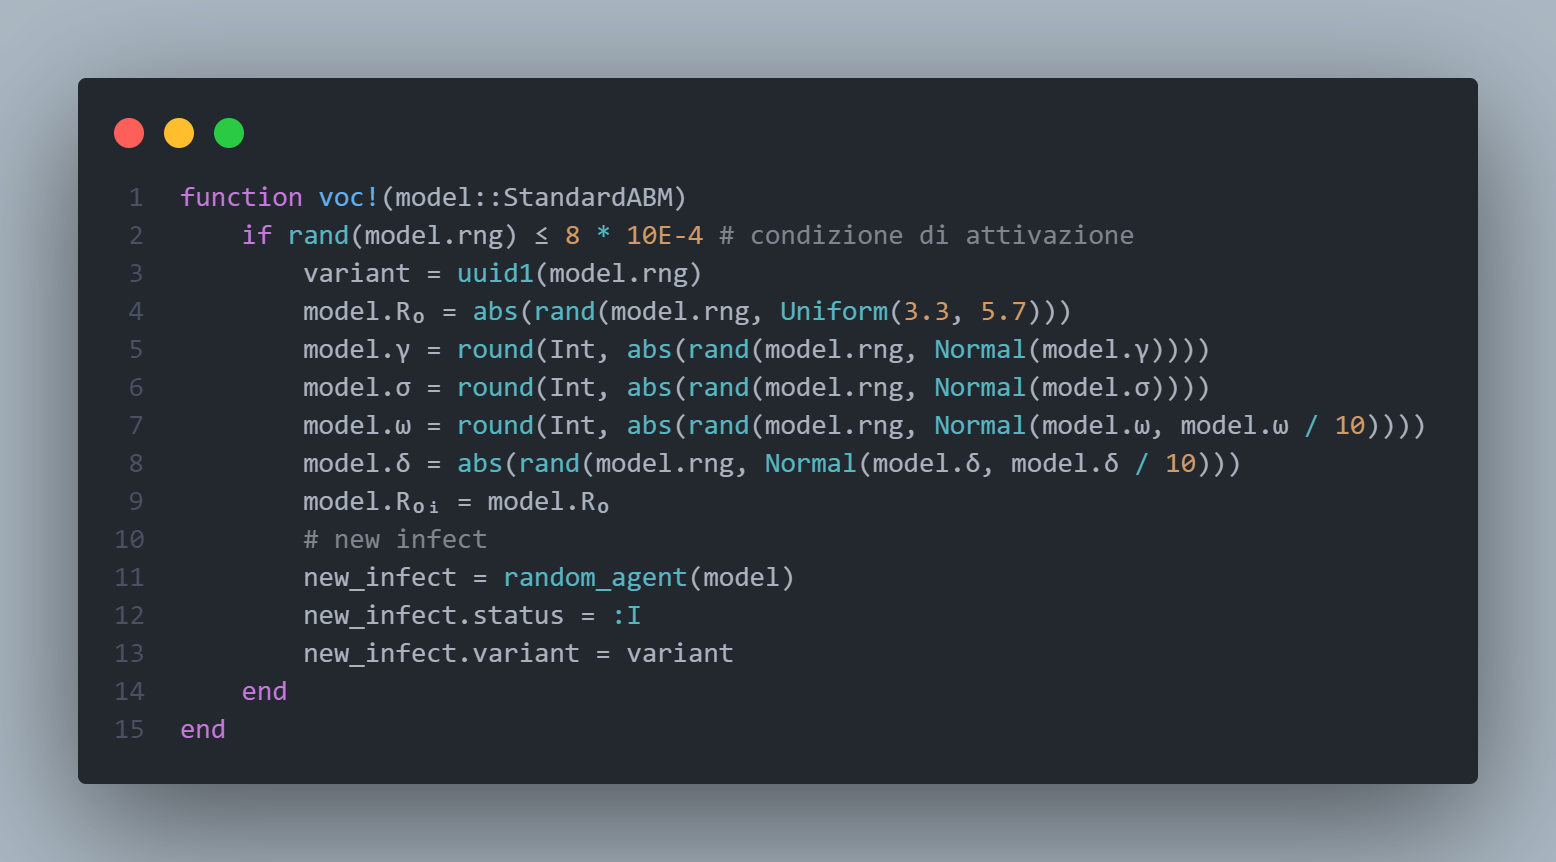
\includegraphics[width=\textwidth]{img/voc.png}
	\captionof{figure}{Funzione che si occupa di generare la VOC}
	\label{fig:voc}
\end{minipage}

\subsubsection{Funzione per la Simulazione della Campagna di Vaccinazione}

La simulazione della campagna di vaccinazione si fonda su un approccio 
in cui viene vaccinata una percentuale fissa di popolazione ad ogni 
passo del modello. Questa percentuale è scelta in modo tale da tenere 
conto dell'obiettivo di raggiungere l'immunità di gregge entro un 
periodo di tempo specifico. Tuttavia, è importante notare che questo 
approccio è basato su alcune assunzioni semplificative, le quali 
comprendono:

\begin{itemize}
	\item \textbf{Effetto delle mutazioni del virus sulla distribuzione
	dei parametri pandemici}: Nel modello, si suppone che le mutazioni 
	del virus possano influenzare la distribuzione dei parametri 
	pandemici, come l'infettività e la gravità dei sintomi. 
	Tuttavia, il modo in cui le mutazioni influenzano questi parametri 
	è approssimato in modo semplificato, mentre nella realtà, 
	le interazioni tra le mutazioni e i parametri pandemici sono 
	estremamente complesse e variabili.
	\item \textbf{Meccanismo di vaccinazione basato su dosi fisse}: Nel 
	contesto della simulazione, il processo di vaccinazione è modellato 
	come somministrazione di dosi fisse di vaccino a una percentuale 
	della popolazione. Questa rappresentazione semplificata non tiene 
	conto di fattori come la distribuzione dei vaccini, la copertura 
	effettiva, la risposta immunitaria individuale e la necessità di 
	dosi di richiamo, che sono elementi importanti nella gestione di 
	una campagna di vaccinazione nel mondo reale.
\end{itemize}

\begin{minipage}{\linewidth}
	\centering
	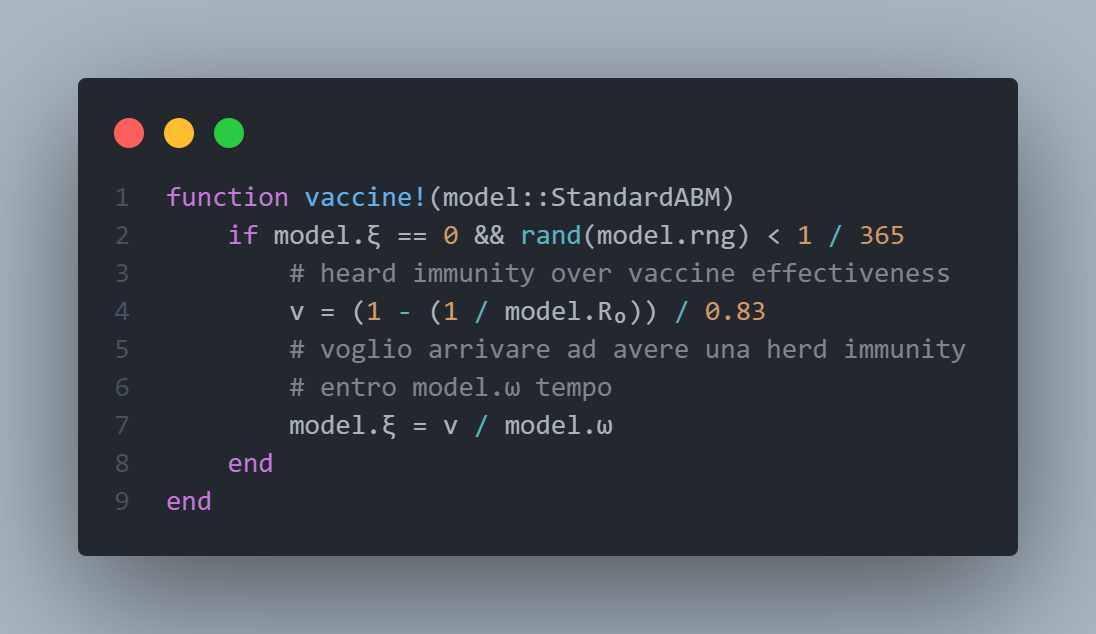
\includegraphics[width=\textwidth]{img/vaccine.png}
	\captionof{figure}{Funzione che si occupa di simulare la ricerca di un vaccino e la sua successiva applicazoine}
	\label{fig:vaccine}
\end{minipage}

Queste semplificazioni nel modello consentono una simulazione più 
gestibile e comprensibile, ma è fondamentale comprendere che non 
riflettono completamente il comportamento complesso e variabile 
del mondo reale. Le simulazioni sono uno strumento utile per l'analisi 
e la previsione, ma devono essere interpretate con consapevolezza delle 
limitazioni delle assunzioni adottate.